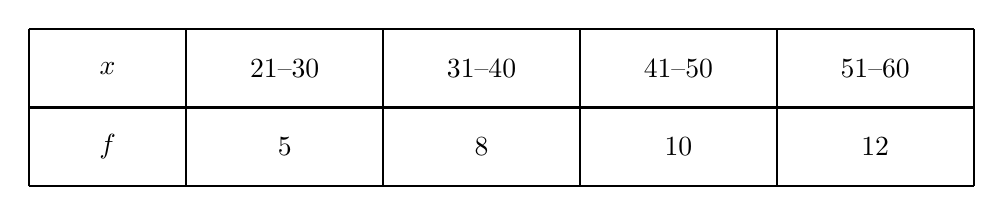
\begin{tikzpicture}[scale=1.0]

    % --- Grid Construction ---
    % Drawing horizontal lines for the table rows
    % Bottom line
    \draw[thick] (0, 0) -- (12, 0);
    % Middle divider line
    \draw[thick] (0, 1) -- (12, 1);
    % Top line
    \draw[thick] (0, 2) -- (12, 2);

    % Drawing vertical lines for the table columns
    % Leftmost border
    \draw[thick] (0, 0) -- (0, 2);
    % First column divider (separating headers x/f from data)
    \draw[thick] (2, 0) -- (2, 2);
    % Second column divider
    \draw[thick] (4.5, 0) -- (4.5, 2);
    % Third column divider
    \draw[thick] (7, 0) -- (7, 2);
    % Fourth column divider
    \draw[thick] (9.5, 0) -- (9.5, 2);
    % Rightmost border
    \draw[thick] (12, 0) -- (12, 2);

    % --- Content Labels ---
    
    % Row 1: Headers and Ranges (centered vertically at y=1.5)
    % Label 'x' in the first column
    \node at (1, 1.5) {$x$};
    % Range 21-30
    \node at (3.25, 1.5) {21--30};
    % Range 31-40
    \node at (5.75, 1.5) {31--40};
    % Range 41-50
    \node at (8.25, 1.5) {41--50};
    % Range 51-60
    \node at (10.75, 1.5) {51--60};

    % Row 2: Values (centered vertically at y=0.5)
    % Label 'f' in the first column
    \node at (1, 0.5) {$f$};
    % Value 5
    \node at (3.25, 0.5) {5};
    % Value 8
    \node at (5.75, 0.5) {8};
    % Value 10
    \node at (8.25, 0.5) {10};
    % Value 12
    \node at (10.75, 0.5) {12};

\end{tikzpicture}